\documentclass[conference]{IEEEtran}
\usepackage[pdftex]{graphicx}
\usepackage{amsmath}
\usepackage{booktabs}
\usepackage{xcolor}
\usepackage{listings}
\lstset{basicstyle=\ttfamily,
	showstringspaces=false,
	commentstyle=\color{red},
	keywordstyle=\color{blue}
}
\usepackage{biblatex}
\usepackage[colorlinks=true,allcolors=black]{hyperref}
%\usepackage[backend=biber, bibencoding=utf8, style=ieee]{biblatex}
\addbibresource{references.bib}

\begin{document}
\title{Practical Report Group 14: Broker\\ {\fontsize{13}{0}\selectfont Internet of Things (2IMN15) 2016-2017, Eindhoven University of Technology} \\ {\fontsize{13}{0}\selectfont \today }}

\author{\IEEEauthorblockN{Sai Krishna Kalluri}
	\IEEEauthorblockA{TU/e, Netherlands\\
		Email: saikrishh.kalluri@gmail.com}
	\and
	\IEEEauthorblockN{Snorri Stefansson}
	\IEEEauthorblockA{TU/e, Netherlands\\
		Email: snorriste@gmail.com}}
\maketitle

\IEEEpeerreviewmaketitle


\begin{abstract}
	This practical assignment for the course IoT involves creating a lightning system controlled and managed by different but relevant wireless protocols and separated individual applications. The architecture and development of this system will be the topic of this report.\\
	
\end{abstract}

\section{Group Members}

\section{Group Partners}




\section{System Description - Understanding the application}

Creating a lighting system with an IoT architecture may sound like an overkill, yet when the application and architecture is designed carefully it becomes essential in everyday life. This system will be described as it will be tested in the final plug fest of this course. The light system is composed of; four lights, each with a user, a user application with a UI, a sensor to detect the users presence, a manager, his web manager UI. These are the most important physical components which allow for a complete system to be operated. There are three groups which develop this system as stated in Figure \ref{fig:fig1}.

\begin{figure}[h]
	\begin{center}
		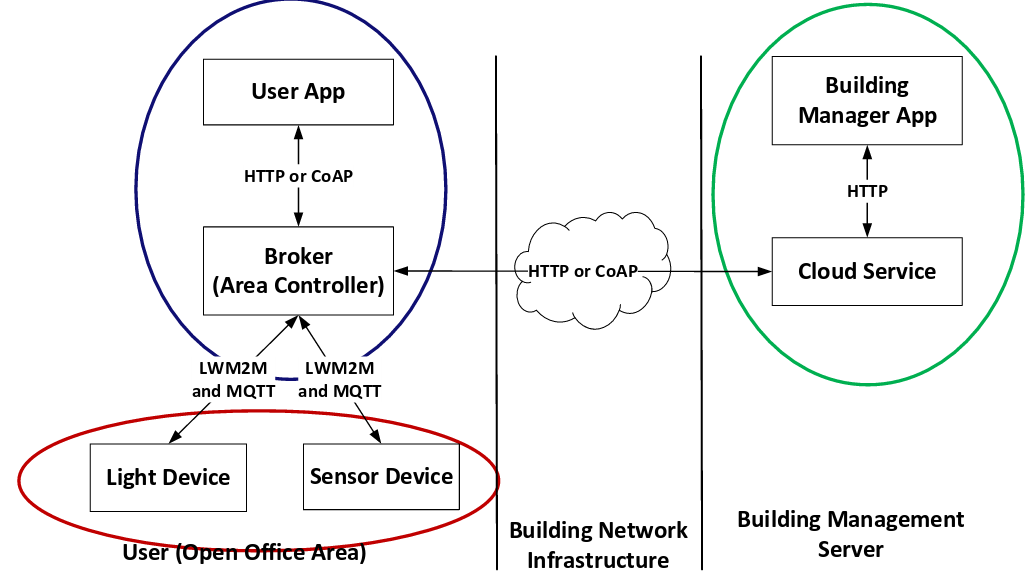
\includegraphics[width=1\linewidth]{img/design}
		\caption{This Figure is from the lecture slides on IoT \cite{slides}}
		\label{fig:fig1}
	\end{center}
\end{figure}

\section{System Interfaces}

Each team has their purpose. This is the report of the broker, thus will be written with that perspective. Two other teams complete the total assignment, they are cloud group and end-device group and will be references as that through out the report. To shortly describe the relationship with these groups and their purpose; The cloud group is basically responsible of bookkeeping of all information important for the system and the end-device group is responsible of maintaining lights and sensors in the systems which define end device. The end device will present light upon request of the user and be able to detect a user with a camera, sensor.

\section{Implementation, Architecture and Protocols}

There are four significant deliverables for the broker group. Each of them 
\begin{enumerate}
	\item There is a user app for the user to control the light/s, which was selected to be a Android app for this showcase.
	\item mDNS discovery service. Avahi was chosen for this job and is built into linux or can be used with python for integration into a python project.
	\item LWM2M (Rest API) - a 'light weight machine to machine communication' with end device as well as maintaining a CoAP/HTTP server. Leshan was chosen for this task and is written in Java.
	\item MQTT broker which allows lights and sensors to communicate basic commands between one and other with this well suited subscribe and publish service. Mosquitto version 1.4.8 was used for this and installed on linux.
\end{enumerate}

\textit{A laptop with Ubuntu 16.04 64-bit was used to run all these modules except the Android app which was run with an emulator and designed on a Windows computer.}

The architecture is somewhat predefined but many design options were left up to the teams. All communication and information will pass through the broker on its way to the endpoint.

\begin{figure}[h]
	\begin{center}
		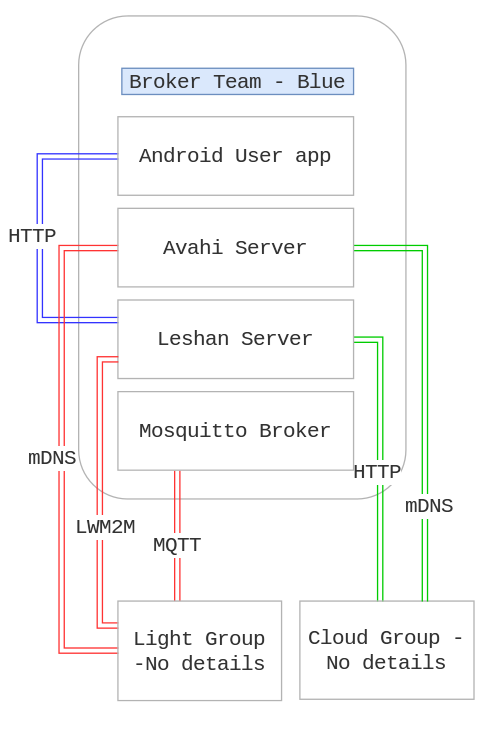
\includegraphics[width=0.8\linewidth]{img/overview}
		\caption{}
		\label{fig:fig2}
	\end{center}
\end{figure}

\subsection{LWM2M: CoAP and HTTP with Leshan}


LWM2M is the fundamental ingredient in the broker. It provides a REST API for both CoAP and HTTP which can both be modified to serve the needs of the system. Leshan operates with a server/client infrastructure. Thus the broker runs a server module and other devices connecting to it use a client module. The android app and the cloud service take advantage of the HTTP protocol and the end-device uses the CoAP protocol.


\subsection{User app: Android}

\subsection{mDNS: Avahi broker}
This part 

\subsection{MQTT: Mosquitto}


\begin{figure}[h]
	\begin{center}
		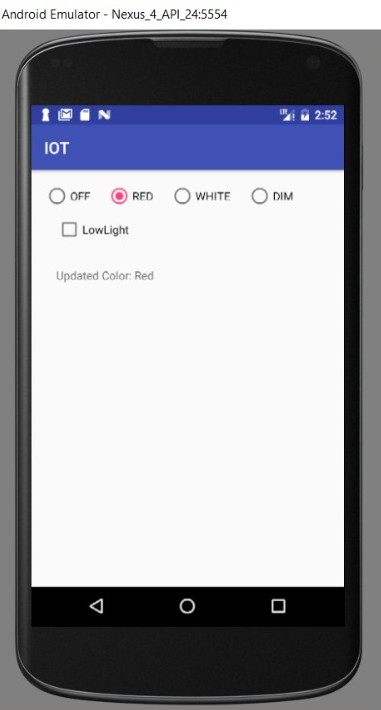
\includegraphics[width=.7\linewidth]{img/androidapp}
		\caption{}
		\label{fig:fig3}
	\end{center}
\end{figure}


\section{Product Testing}

From day one all code had to be tested frequently and thoroughly, eliminating errors and all bad test cases. Most testing had to be done with the Leshan server. A dummy client was created to simulated the end device and then HTTP request where sent from browser and tested with the android app as well.

\subsection{MQTT testing}

Testing was done on MQTT for making sure that clients could connect to it and communicate the FREE/OCCUPIED between the sensor and light device. That part worked for all teams connecting to the system. As can be seen in Figure \ref{fig:mqtt3}.
\begin{figure}[h]
	\begin{center}
		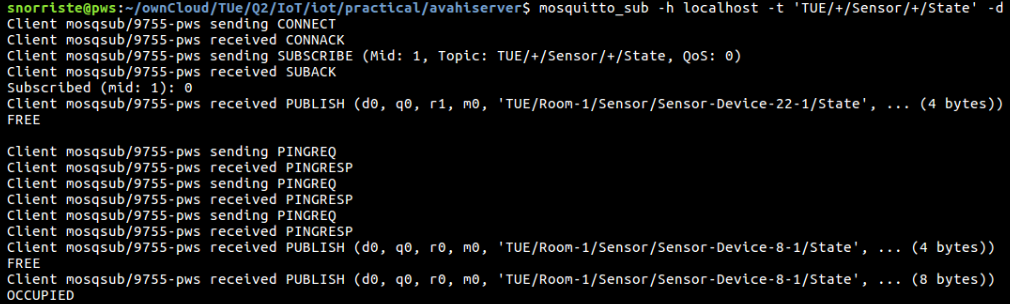
\includegraphics[width=\linewidth]{img/mqtt3}
		\caption{Mosquitto tested during Plugfest with other teams. MQTT broker works and clients can communicate.}
		\label{fig:mqtt3}
	\end{center}
\end{figure}

\subsection{Leshan Testing}

This section will show testing of Leshan, how it responded to requests and how the development interface looks like. In Figure \ref{fig:observe} the log for the Leshan server is displayed when an request from the web app is made to observe a sensor value (resource 10350).

\begin{figure}[h]
	\begin{center}
		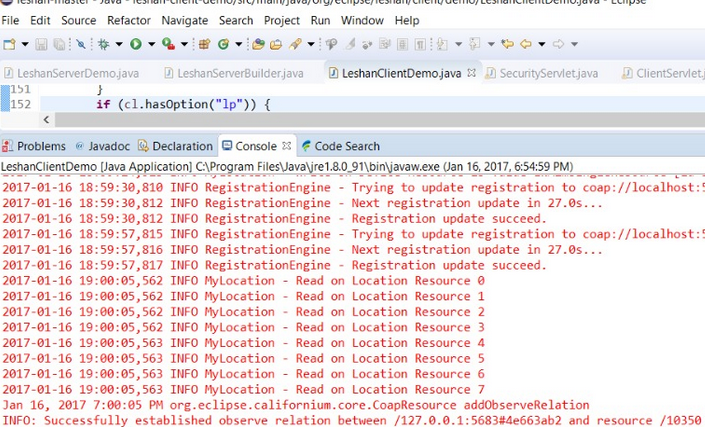
\includegraphics[width=\linewidth]{img/screenshot-observe}
		\caption{It can be seen here that an observation was made on an resource}
		\label{fig:observe}
	\end{center}
\end{figure}

An important part to be working is the updating of ownership and thus it is useful to show the testing of the part. In Figure \ref{fig:own} the Leshan server log can be seen when the Cloud group updates the ownership via their manager web app seen in Figure \ref{fig:cloudown}.

\begin{figure}[h]
	\begin{center}
		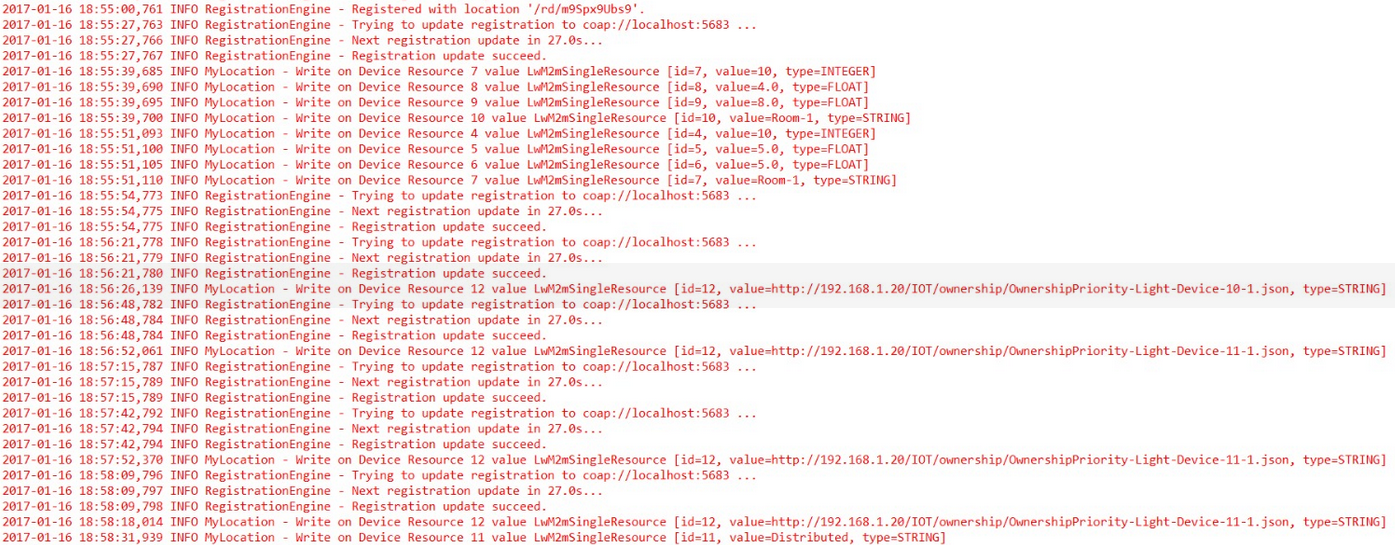
\includegraphics[width=1.18\linewidth]{img/screenshot-ownership}
		\caption{Here it can be seen that the ownership was updated from another IP address, namely the Cloud}
		\label{fig:own}
	\end{center}
\end{figure}

\begin{figure}[h]
	\begin{center}
		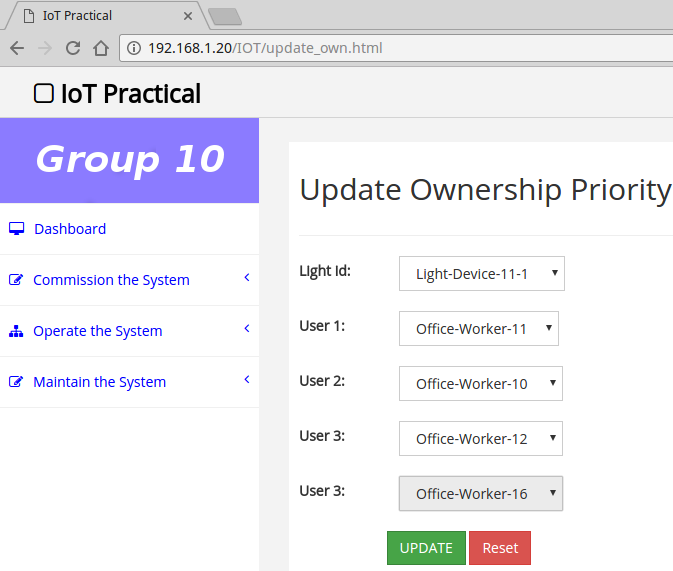
\includegraphics[width=.8\linewidth]{img/screenshot-cloud-ownership}
		\caption{The Cloud group updates the ownership in the Leshan server via their web app in this picture. The IP matching the IP in the logs in Figure \ref{fig:own}}
		\label{fig:cloudown}
	\end{center}
\end{figure}

\subsection{App Testing}
In Figure \ref{fig:app} the app can be seen working with multiple clients. The light can be controlled as indicated.

\subsection{Avahi Testing}

Avahi was tested multiple times with the red team. Figure \ref{fig:avahi} shows the command publish the service and then if the client uses the same parameters it will connect. 
\section{Discussion and results}
\section{Evaluation}

Now the systems has been developed so that it can talk to any end-device with the predefined information sharing. The broker can be turned on, make it self discoverable to any end-device (mDNS), allow for communication between light and sensor device (MQTT) and finally allows for end-devices to register as clients in Leshan and be accessed by the cloud with jetty inside Leshan. This is the complete, simplified, architecture use case.	
\section{Reflection}


\section{Contribution}
\subsection{UserApp(Android)}
begin{enumerate}
\item LoginActivity: Validating the entered user details against server- Snorri.
\item ClientActivity: Collecting information related to current state of the system from broker- SaiKrishna.
\item ControlActivity: Creating User interface for light objects-Snorri
\item  ControlActivity: Communicating the updated light state to the broker- Sai Krishna.
\item Utilities:Creating and handling HTTP requests,parsing JSON information from server-Sai Krishna.
end{enumerate}

\subsection{Server(Leshan)}
begin{enumerate}
\item ClientServlet:Handling read, write and observation requests from cloud and UserApp-Snorri
\item EventServlet:Performing operations during registrations, creating new observation requests- Sai Krishna

\item EventServlet(CentralizedDeployment):Handling new observations,updating databases,centralized Deployment routine-Snorri

\item Security Servlet:Storing User details received from cloud and handling Login validation requests from UserAPP- Sai Krishna.

\item Utilities:Json parsing,Dummy Clients for testing-Sai Krishna

\subsection{Avahi}-Creating network discovery for both clients and cloud service-Snorri.
\subsection{MQTT}-Creatig MQTT broker client publish and subscriptions -Snorri.

\subsection{Report} Report for the project-Snorri and Sai Krishna.




\printbibliography

\end{document}